\chapter{Implementation}
This chapter deals with the details of the \emph{slicevis} package implementation. First, a brief overview of the user interface is given and then the internal methods and logic is laid out.

To build the interactive GUI, \emph{slicevis} relies on several other packages, namely jupyter, ipywidgets, and plotly .  

The \texttt{widget.py} modules defines the \texttt{SliceWidget} class which constructs the GUI and handles all user interaction. A three-dimensional NumPy \texttt{ndarray} is passed to the class instance constructor \cite{ndarray}. There is also an optional debug mode which enables an Output widget  and layout borders for developers. The init method adds all buttons, creates layouts, and connects function callbacks. Each widget has at least one callback associated to it.

\begin{figure}[h]
	\centering
	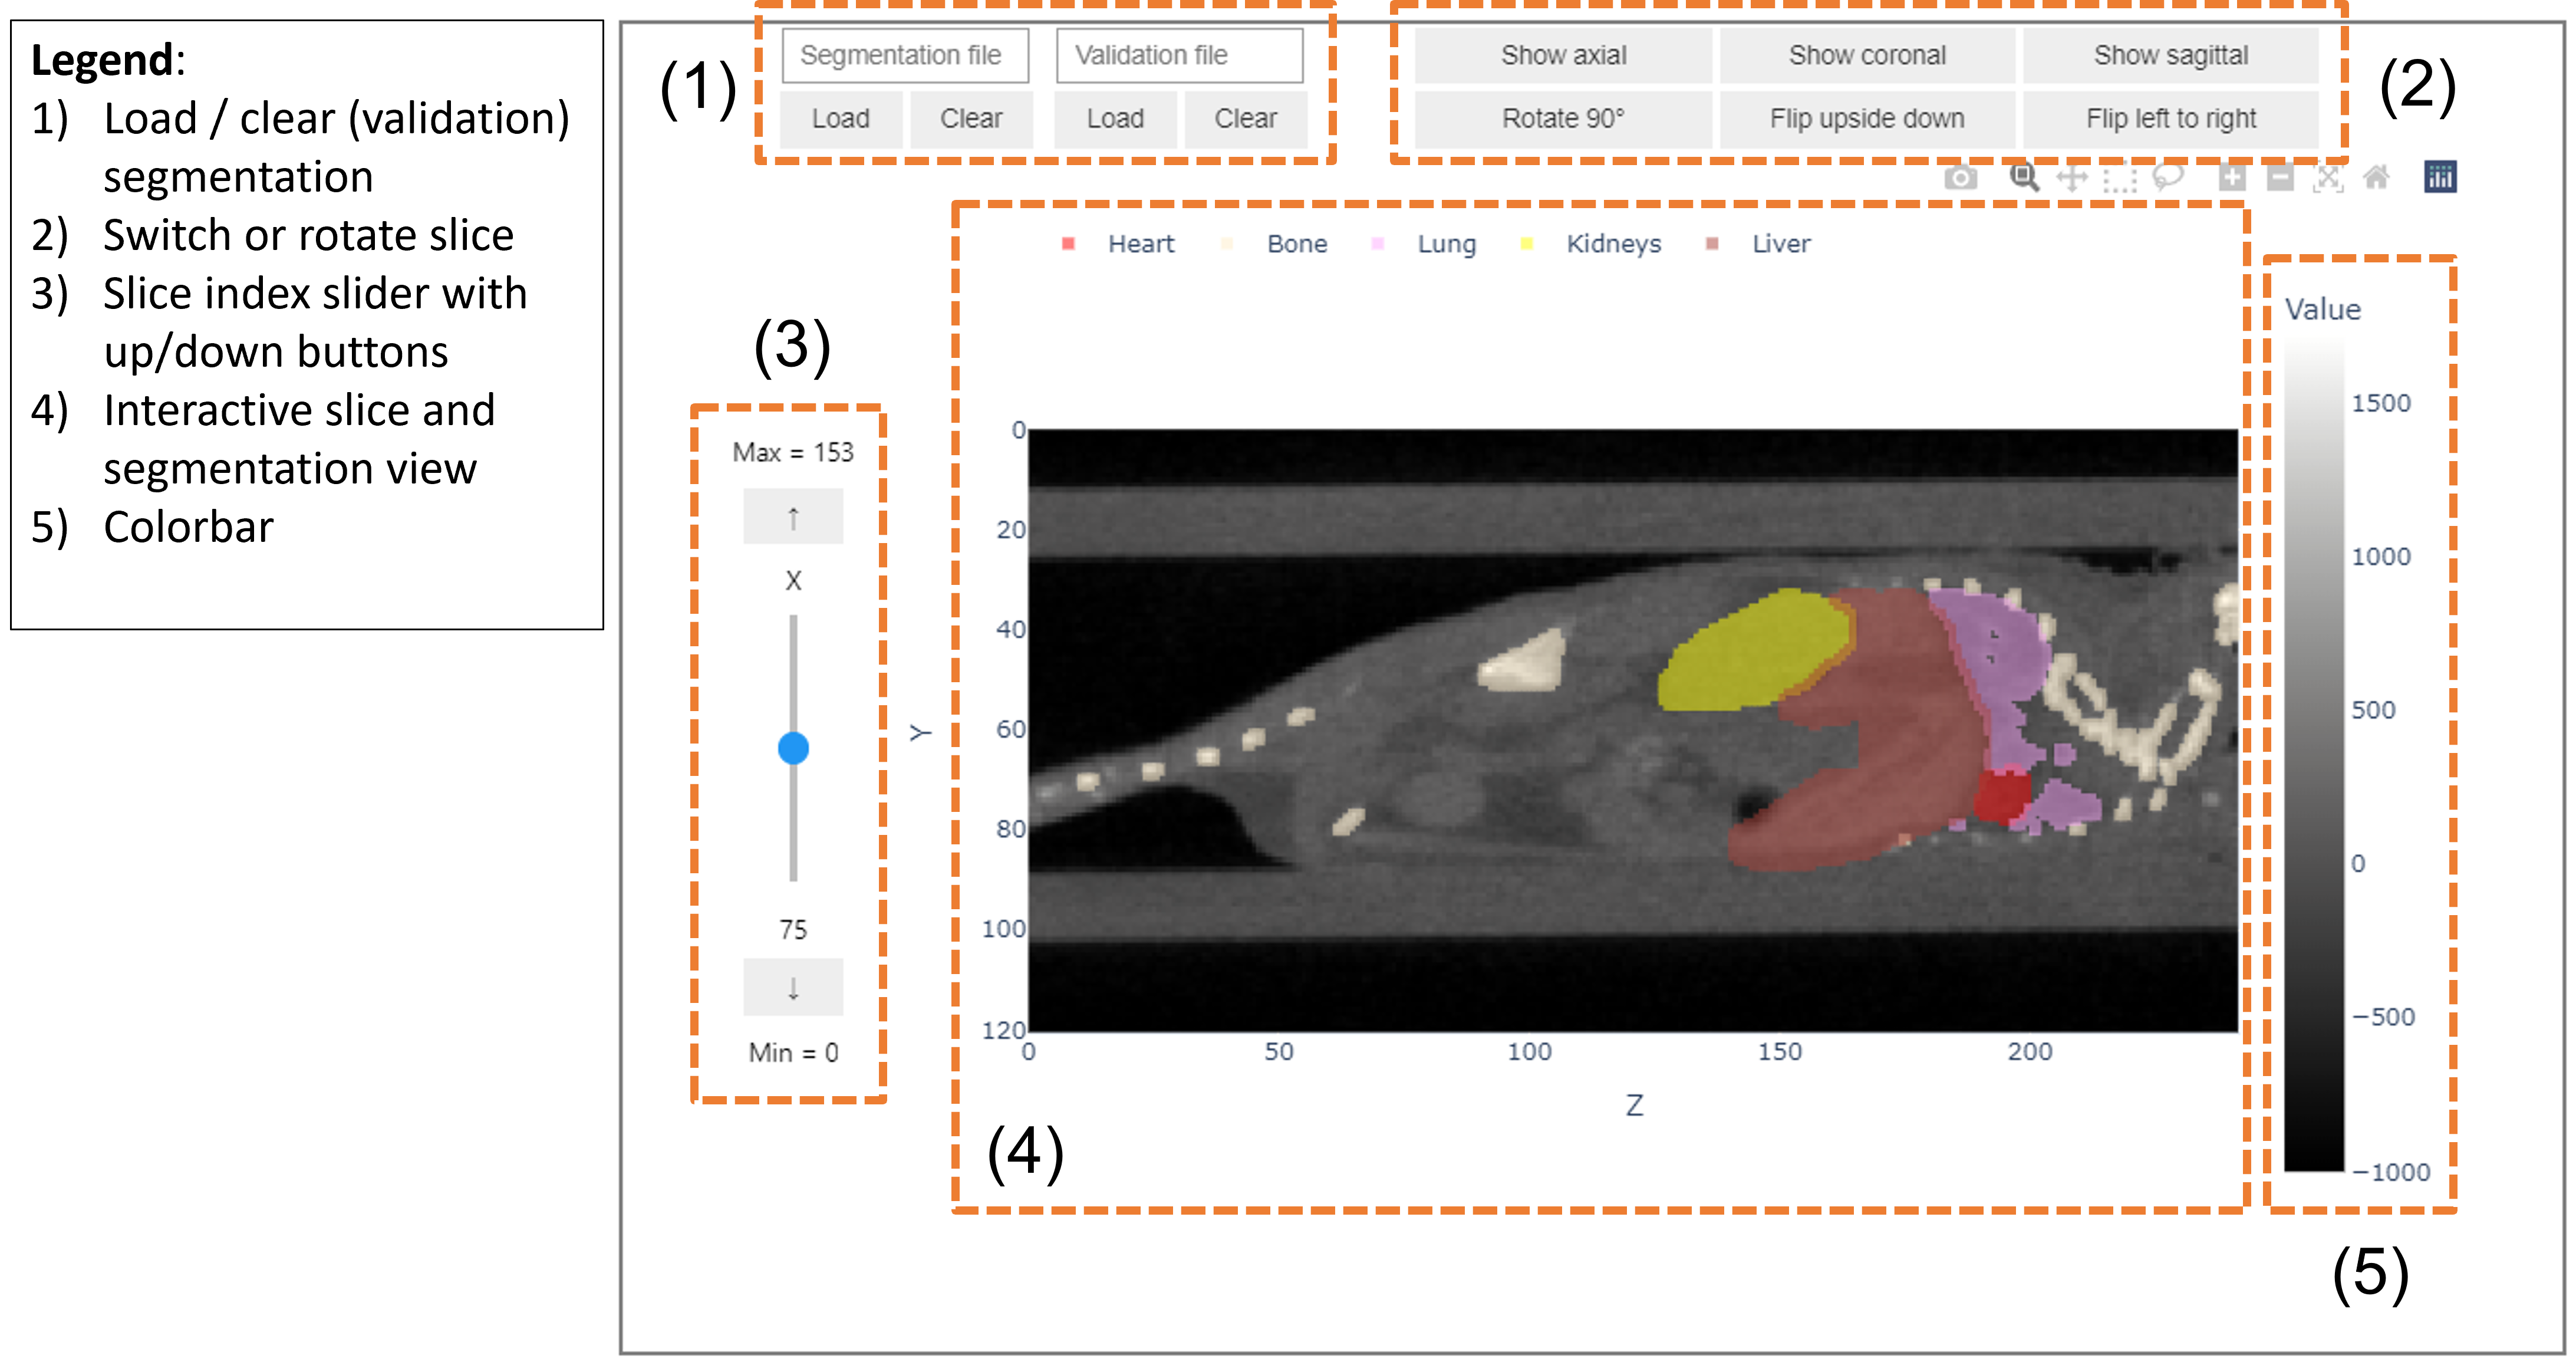
\includegraphics[width=.9\linewidth]{figures/GUI.png}
	\caption{The SliceWidget GUI, annotated.}
\end{figure}

Internally, the \_update2D method is the most important function as it responsible for setting the 2D image to the correct slice each time the user interacts with the widget. \_update2D also paints the (up to) two segmentations as scatter plots on top of the image. As this method is called multiple times per second for smooth slicing, it must be reasonably efficient in its implementation. Updating the 2D image is as simple as indexing into the (possibly rotated) 3D image in the current axis where the index is given as input to the callback. What is more tricky is painting the segmentations with their class names and colors on top. To find the pixels with coordinates $(x_i , y_i)$ of the class with index $j$ in the current slice, the Numpy method \emph{nonzero(condition)} is used. As \emph{condition}, one can ask where \emph{self.seg2D} $== j$. With the list of coordinate pairs, the class name, and its color, it is then possible to create a Plotly Scatter object and append it to the trace list. This is repeated for each segmentation class. In the end, a \emph{batch\_update()} is called on the widget where the 2D image is swapped out and the trace list is added on top. By batching the updates to the widget the render engine performs them all at once and flickering or delays are minimized. 

\begin{figure}[h]
	\centering
	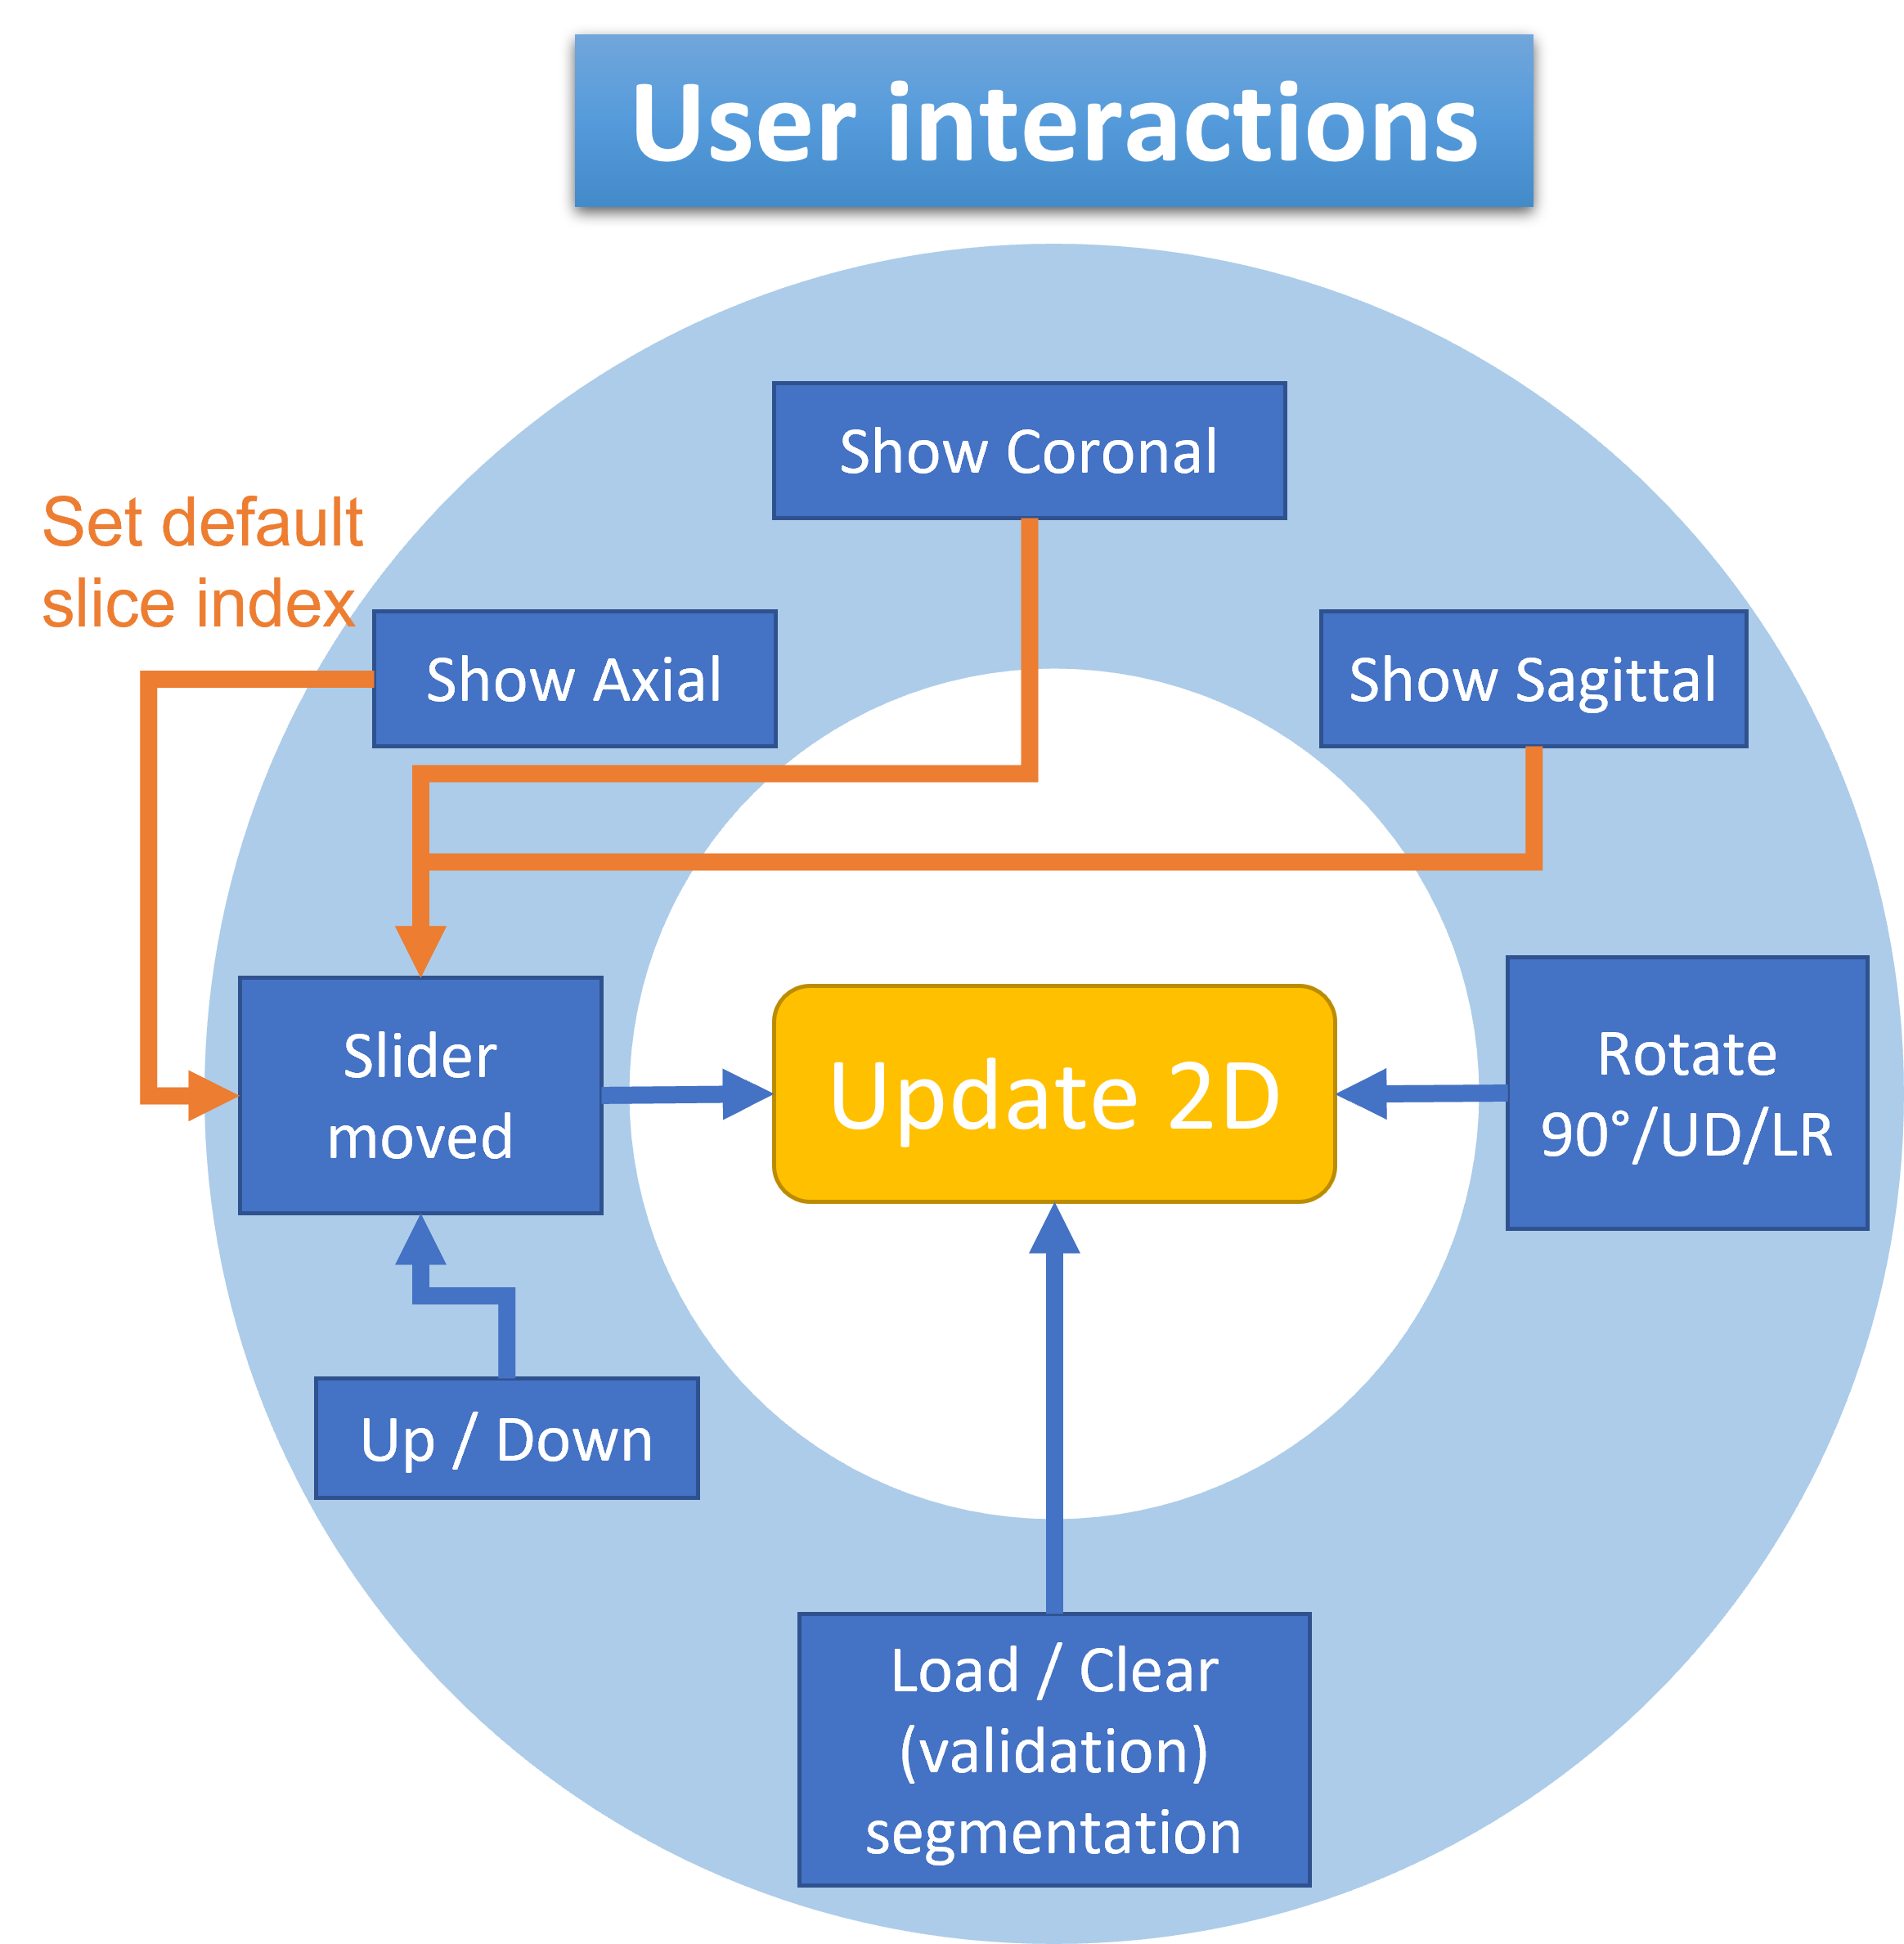
\includegraphics[height=.5\linewidth]{figures/call_graph.png}
	\caption{Call graph for interactive GUI update.}
\end{figure}

For more details, please refer to the documentation in the code.

DICE score computation:

\begin{equation}
	DICE(X, Y) =\frac{2|X \cap Y|}{|X|+|Y|}
\end{equation}